\documentclass[11pt,letterpaper]{article}

\usepackage[margin=1in]{geometry}
\usepackage[T1]{fontenc}
\usepackage[utf8]{inputenc}
\usepackage{microtype}
\usepackage{amsmath,amssymb}
\usepackage{booktabs}
\usepackage{graphicx}
\usepackage{caption}
\usepackage{authblk}
\usepackage{enumitem}
\usepackage[hyphens]{url}
\usepackage{xcolor}
\usepackage[round,authoryear]{natbib}
\usepackage{hyperref}
\usepackage{../../tex/monterey}

\hypersetup{
  pdftitle={Post-Earnings Announcement Drift under AAOIFI Screens: An Exploratory Backtest of Halal Earnings Surprise, 2020-2025},
  pdfauthor={Rao Abdul Hadi},
  pdfsubject={Halal equity investing, PEAD, SUE, earnings surprise, AAOIFI screens},
  pdfkeywords={PEAD, SUE, earnings surprise, AAOIFI, Sharia-compliant equities, post-earnings announcement drift, backtest},
  colorlinks=true,
  citecolor=blue,
  linkcolor=blue,
  urlcolor=blue
}

\captionsetup{font=small,labelfont=bf,skip=6pt}
\setlength{\parindent}{1.5em}
\setlength{\parskip}{0pt}
\setlist[itemize]{leftmargin=1.5em,itemsep=0.2em,topsep=0.35em}
\setlist[enumerate]{leftmargin=1.5em,itemsep=0.2em,topsep=0.35em}

\renewcommand\Authfont{\normalsize}
\renewcommand\Affilfont{\small}
\setlength{\affilsep}{0.6em}

\title{\textbf{Post-Earnings Announcement Drift under AAOIFI Screens:\\
An Exploratory Backtest of Halal Earnings Surprise, 2020--2025}}

\author[1]{Rao Abdul Hadi\thanks{Corresponding author. Email: \href{mailto:raoabdulhadi952@gmail.com}{raoabdulhadi952@gmail.com}. This is an unrefereed working paper. It has not been peer reviewed.}}
\affil[1]{Monterey Finance, Halal Quant Research Lab}

\date{September 2026}

\begin{document}
\maketitle

\begin{abstract}
\noindent
This paper asks whether post-earnings announcement drift (PEAD) still appears after Islamic business and leverage screens, and whether it is weaker than the same rule on broad S\&P~500 constituents. I start from the current S\&P~500, drop banned activities, keep names whose standardized unanticipated earnings (SUE) exceed two robust standard deviations of that stock's own prior forecast errors, enter on the first session after the print, equal-weight, and hold for 21 trading days. From 31~January~2020 through 30~December~2025 the Halal book returned 27.7\% compound annual growth, against 15.1\% for SPY, 13.4\% for the S\&P~500 index, and 17.7\% for a Halal large-cap ETF (SPUS). A broad-index twin---same SUE rule, no AAOIFI overlay---returned 28.6\% CAGR. Mean cumulative abnormal return versus SPY after qualifying prints is $+1.01\%$ at 21 days and $+1.58\%$ at 60 days in the Halal sleeve, versus $+1.44\%$ and $+1.82\%$ in the full index. Event-time SUE quintiles inside Halal names are ordered: Q5 compounds at 28.2\% while Q1 is $-1.5\%$. A first specification that cap-weighted a 60-day window at month-end lagged both benchmarks (13.4\% CAGR) because it bought stale mega-cap beats after the gap had already printed. The sample is a large-cap Yahoo earnings calendar, about 16\% of prints still clear a nominal $2\sigma$ cutoff, turnover is high, and 2025 lagged SPUS. The numbers should be read as an exploratory backtest, not as a forecast or a live-return target.
\end{abstract}

\noindent\textbf{Keywords:}
PEAD; standardized unanticipated earnings; earnings surprise; AAOIFI; Sharia-compliant equities; post-earnings announcement drift; backtest.

\noindent\textbf{JEL classification:} G11, G12, G14, Z12.

\noindent\textbf{Code:}
Replication notebook and figures are in the Monterey Finance repository,
\url{https://github.com/regional-specter/Monterey-Finance},
under \path{Research/papers/06-earn-momentum-sue/}.
First-pass figures are archived in \path{figures/Run 1/}.

\section{Introduction}

Markets do not fully digest earnings news on announcement day. Standardized unanticipated earnings (SUE)---actual EPS minus consensus, scaled by the stock's own history of forecast errors---predict subsequent returns for weeks \citep{ball1968,foster1984,bernard1989,bernard1990}. That post-earnings announcement drift (PEAD) is one of the most replicated anomalies in U.S.\ equities. The open question for this lab is narrower. After AAOIFI activity and financial-ratio screens remove banks, highly indebted issuers, and other non-compliant businesses \citep{aaoifi21,derigs2008}, does the same $2\sigma$ surprise still drift, and does it drift less than in the unscreened index?

Sharia screens change who can print a usable surprise. They cut conventional financials, where earnings news is frequent and often well covered, and they leave more operating firms in technology, healthcare, and industrials. If PEAD is mainly a small-stock, low-coverage effect, a Halal S\&P~500 sleeve might show little drift. If PEAD is simply delayed processing of public earnings news, Halal and broad books should look similar once the portfolio is built to match the event study.

The first live book in this project did not match the event study. It rebalanced at month-end, cap-weighted, and held names for 60 trading days. Event-study CAR after SUE$>2\sigma$ prints was positive, but the portfolio lagged SPY and SPUS. Inspection showed the book was mostly mega-caps 36--48 days after the print, with GOOG and GOOGL both weighted, and SUE quintiles inverted. That specification is archived as Run~1. The live rule tested here is the repair: robust SUE, share-class collapse, equal weight, first session after the announcement, 21-day hold.

On that rule the Halal PEAD book beat both benchmarks and tracked the broad PEAD twin closely. Drift is a little weaker after AAOIFI compliance than in the full index, but it is not gone. Quintiles now reward higher SUE. Costs, sparse holdings, and a weak 2025 are first-order caveats. I treat the result as evidence that PEAD can be implemented under Halal screens if the book is event-time, not as proof that a $2\sigma$ cutoff is a cycle-proof factor.

The rest of the paper is organized as follows. Section~\ref{sec:data} describes the universe, screens, and SUE definition. Section~\ref{sec:rules} states the live portfolio rules. Section~\ref{sec:revision} documents the Run~1 failure and the specification change. Section~\ref{sec:results} reports live-window performance, calendar years, the event study, and quintiles. Section~\ref{sec:attrib} looks at Halal versus broad, sector mix, and holdings. Section~\ref{sec:limits} covers turnover, data limits, and what would be required before a live mandate. Section~\ref{sec:conc} concludes.

\section{Data, screens, and signal definitions}
\label{sec:data}

\subsection{Universe}

The starting list is the current S\&P~500 (503 tickers). A one-time activity screen removes 64 names (conventional banking and insurance, tobacco, defense, and similar businesses), leaving 439 sector-eligible stocks. Financial-ratio screens then re-run on the latest month-end AAOIFI snapshot on or before each holding day. I use the \texttt{halalquant} library: debt below 30\% of market cap, with the library's cash and receivables caps. Compliance is a hard constraint. A name that fails on a holding day is not held.

The price sample is 1~January~2020 through 31~December~2025, with extra price and earnings history from mid-2018 so that $\sigma$ and the 21-day window are defined. Performance statistics begin on the first day the strategy actually holds stocks, 31~January~2020, and run through 30~December~2025 (1{,}487 trading days). Days before that first invested date are omitted, not filled with zeros.

Yahoo had missing in-sample prices for a handful of tickers (including FDXF, HONA, and a failed AMZN pull on this run). Those names are skipped where data are missing. The S\&P list is current membership, not a point-in-time file, so the universe has survivorship.

\subsection{Screening standard}

The financial screens follow AAOIFI ratios, not the Dow Jones Islamic Market (DJIM) thresholds \citep{aaoifi21,derigs2008}. SPUS (SP Funds S\&P~500 Sharia Industry Exclusions) is the Halal index comparison. It is a cap-weighted, industry-exclusion ETF. It is not identical to a pure AAOIFI financial-ratio index. SPY is the tradable all-stock benchmark; \texttt{\^{}GSPC} is the S\&P~500 cash index.

The broad PEAD twin uses the same SUE rule on the raw index list, with no AAOIFI overlay at selection. That is the white-paper contrast: Halal equities versus broad index constituents.

Table~\ref{tab:universe} summarizes the design choices.

\begin{table}[htbp]
\centering
\caption{Universe, screens, and sample.}
\label{tab:universe}
\begin{tabular}{ll}
\toprule
Item & Choice \\
\midrule
Target factor & Robust SUE $> 2$; positive earnings beat \\
Starting universe & Current S\&P~500 list (503 tickers) \\
After banned-business screen & 439 tickers (64 removed) \\
Screening standard & AAOIFI financial ratios, not DJIM \\
Halal benchmark & SPUS (SP Funds S\&P~500 Sharia Industry Exclusions) \\
All-stock benchmarks & SPY; S\&P~500 (\texttt{\^{}GSPC}) \\
Contrast book & Same SUE rule on unscreened index names \\
Sample requested & 1~Jan~2020 -- 31~Dec~2025 \\
Live window used for stats & 31~Jan~2020 -- 30~Dec~2025 (1{,}487 trading days) \\
\bottomrule
\end{tabular}
\end{table}

\subsection{Standardized unanticipated earnings}

For each quarterly print with both reported EPS and a consensus estimate,
\[
e_{i,t} =
\begin{cases}
\text{Yahoo surprise (\%)} & \text{if at least six prior \% surprises exist,} \\
EPS_{i,t} - \widehat{EPS}_{i,t} & \text{otherwise.}
\end{cases}
\]
SUE is that error scaled by a \emph{robust} prior-error standard deviation:
\[
\sigma_{i,t}
= \max\bigl(
\widehat{\sigma}_{i,t}^{5/95},\;
\tfrac{1}{2}\operatorname{median}|e_{i,<t}|,\;
10^{-8}
\bigr),
\qquad
\mathrm{SUE}_{i,t} = \frac{e_{i,t}}{\sigma_{i,t}},
\]
where $\widehat{\sigma}^{5/95}$ is the sample standard deviation of prior errors after winsorizing at the 5th and 95th percentiles. The floor stops a compressed pre-period (for example 2019 errors before 2020 COVID beats) from minting fake $10\sigma$ observations. A name enters only if $\mathrm{SUE}>2$ \emph{and} the raw beat is positive.

Yahoo earnings dates supply actual and estimated EPS. Prints missing either side are dropped. Dual listings map to one ticker (\texttt{GOOGL}$\to$\texttt{GOOG}, and analogous FOX/NWS pairs).

In the live window there were 11{,}633 dated prints with a usable SUE, of which 1{,}857 (16.0\%) cleared SUE$>2$. Under a Gaussian one-sided $2\sigma$ rule one would expect about 2.3\%. The cutoff is still too loose relative to textbook $\sigma$, even after the robust floor. I keep SUE$>2$ because that is the stated screen; I do not pretend it is a rare tail event in this calendar.

\section{Portfolio rules}
\label{sec:rules}

Rules are event-time. There is no month-end sort of ``who beat last quarter.'' There is no intra-day stop-loss and no single-name cap beyond equal weight.

\subsection{Pipeline}

\begin{enumerate}
  \item Score each print with robust SUE when the announcement is public.
  \item Keep prints with SUE $> 2$ and a positive beat.
  \item Enter on the first trading session \emph{after} the announcement date (the overnight gap is in the event study as day~1; the live book owns days 1--21).
  \item Equal-weight all names still inside the 21-session window that pass the latest AAOIFI snapshot (Halal book) or that have a usable market cap (broad book).
  \item Exit after 21 trading days, or sooner if the name fails AAOIFI on a later snapshot.
\end{enumerate}

If the eligible set is empty, the book earns 0\% that day once it has been live. Statistics start on the first invested date.

\begin{table}[htbp]
\centering
\caption{Entry, exit, and risk limits (live rule).}
\label{tab:rules}
\small
\begin{tabular}{lp{0.62\textwidth}}
\toprule
Rule & Specification \\
\midrule
Entry & First session after a SUE$>2$ print with a positive beat \\
Hold & 21 trading days \\
Weight & Equal weight \\
Share classes & Collapse dual listings to one ticker \\
Intra-month stop-loss & None \\
Position cap & None beyond equal weight \\
Cash when empty & 0\% once live; missing before first print \\
Contrast twin & Same events, no AAOIFI overlay \\
\bottomrule
\end{tabular}
\end{table}

At the last AAOIFI date (31~December~2025) only one Halal name still sat inside the 21-day window (SUE 4.14, 17 days after the print). That is expected: earnings cluster, then the book thins until the next cycle. Across membership-change dates the Halal book held a median of 14 names (minimum 1, maximum 107). The 107 peak is the 2020 COVID print wave.

\section{Specification revision: why Run~1 failed}
\label{sec:revision}

The economic hypothesis never changed. The first implementation did. Run~1 held every SUE$>2$ name still inside a 60-day window, cap-weighted, and updated weights only at month-end. The event study on that run was already positive: about $+0.85\%$ mean CAR on day~1 and $+1.60\%$ by day~60 in Halal names. The live book still returned only 13.4\% CAGR, below SPY (15.1\%) and SPUS (17.7\%). Four construction errors explain the gap.

\paragraph{Stale entry.}
Month-end rebalance bought names 1--60 days after the print. On 31~December~2025 the Run~1 book still had GOOG, GOOGL, and MSFT at 42 days post-print and about 65\% of weight. Halal mean CAR was essentially flat from day~5 ($+0.96\%$) to day~21 ($+0.94\%$). The portfolio owned the dead part of the window.

\paragraph{Cap-weighting.}
PEAD in the literature is stronger in smaller names \citep{bernard1989}. Cap-weighting an S\&P~500 surprise book is a mega-cap overlay.

\paragraph{Double-counted share classes.}
GOOG and GOOGL were separate lines with almost identical SUE, so Alphabet was counted twice.

\paragraph{A broken $\sigma$.}
About 19.5\% of Run~1 prints cleared SUE$>2$. Tiny historical forecast-error denominators turned ordinary beats into extreme SUE. Quintiles of that signal were inverted: Q1 CAGR 18.0\%, Q5 CAGR 15.3\%.

Figure~\ref{fig:run1eq} is the Run~1 equity curve. Figure~\ref{fig:equity} is the live rule on the same 2020--2025 window. The contrast is the point of keeping the archive: PEAD was in the data; the first book did not harvest it.

\begin{figure}[htbp]
\centering

\includegraphics[width=0.88\textwidth]{{figures/Run 1/equity-curves}.png}
\caption{Run~1 (archived): month-end, cap-weighted, 60-day hold. Halal SUE PEAD finishes below SPUS and in line with or below SPY.}
\label{fig:run1eq}
\end{figure}

\begin{figure}[htbp]
\centering

\includegraphics[width=0.88\textwidth]{{figures/Run 1/quintile-growth}.png}
\caption{Run~1 SUE quintiles inside Halal names in the 60-day window, cap-weighted. Q1 leads Q5: the live $2\sigma$ long book was on the wrong side of a weak sort.}
\label{fig:run1q}
\end{figure}

The live rule keeps SUE$>2$ but changes the harvest: robust $\sigma$, share-class collapse, equal weight, $t+1$ entry, 21-day hold. That is an in-sample rewrite after seeing Run~1. Headline results below are therefore partly a test of whether a known PEAD implementation works under Halal screens, not a frozen discovery.

\section{Empirical performance}
\label{sec:results}

All headline numbers use the live window: 31~January~2020 through 30~December~2025. Sharpe and Sortino use a 2\% risk-free rate. Maximum drawdown is peak-to-trough on the growth curve.

\subsection{Headline results}

\begin{table}[htbp]
\centering
\caption{Live-window performance, 31~Jan~2020 -- 30~Dec~2025.}
\label{tab:perf}
\small
\begin{tabular}{lrrrrrr}
\toprule
Book & CAGR & Vol. & Sharpe & Sortino & Max DD & Calmar \\
\midrule
Halal SUE $>2\sigma$ PEAD     & 27.72\% & 24.53\% & 1.04 & 1.22 & $-38.08\%$ & 0.73 \\
Broad SUE $>2\sigma$ PEAD     & 28.62\% & 24.22\% & 1.08 & 1.34 & $-39.68\%$ & 0.72 \\
S\&P~500 (SPY)                & 15.06\% & 20.85\% & 0.68 & 0.84 & $-33.72\%$ & 0.45 \\
S\&P~500 index                & 13.40\% & 21.04\% & 0.61 & 0.75 & $-33.92\%$ & 0.39 \\
Halal (SPUS)                  & 17.67\% & 21.77\% & 0.76 & 1.01 & $-30.80\%$ & 0.57 \\
\bottomrule
\end{tabular}
\end{table}

The Halal PEAD book beat SPY by about 12.7~points of CAGR and SPUS by about 10.1~points. The broad twin is only about 0.9~points ahead of the Halal book. Halal screens do not kill the strategy in this sample; they also do not create extra alpha relative to running the same events without AAOIFI. Volatility is higher than the benchmarks (24.5\% versus 20.9--21.8\%), and maximum drawdown is deeper ($-38.1\%$ versus $-30.8\%$ for SPUS), largely the 2020 COVID trough.

Growth of \$1 is about $4.24$ for the Halal book (total return 323.7\%), versus $2.29$ for SPY (128.8\%) and $2.61$ for SPUS (161.2\%).

\begin{figure}[htbp]
\centering

\includegraphics[width=0.88\textwidth]{figures/equity-curves.png}
\caption{Growth of \$1 under the live rule (event-time, 21-day hold, equal-weight). Halal and broad PEAD pull away from SPY, the S\&P~500 index, and SPUS after 2022, then give some of that back in 2025.}
\label{fig:equity}
\end{figure}

\subsection{Calendar years}

\begin{table}[htbp]
\centering
\caption{Calendar-year total returns. 2020 is from 31~January.}
\label{tab:calendar}
\begin{tabular}{lrrrr}
\toprule
Year & Halal PEAD & Broad PEAD & SPY & SPUS \\
\midrule
2020 & 24.3\% & 30.8\% & 16.2\% & 21.7\% \\
2021 & 44.9\% & 39.3\% & 28.7\% & 35.6\% \\
2022 & $-11.4\%$ & 6.3\% & $-18.2\%$ & $-22.8\%$ \\
2023 & 64.6\% & 57.4\% & 26.2\% & 34.2\% \\
2024 & 48.4\% & 34.0\% & 24.9\% & 26.5\% \\
2025 & 8.6\% & 8.0\% & 18.6\% & 20.7\% \\
\bottomrule
\end{tabular}
\end{table}

The Halal book led in 2020--2021 and especially 2023--2024. It lost less than SPY and SPUS in 2022. It lagged in 2025 (8.6\% versus 18.6\% for SPY and 20.7\% for SPUS). Rolling 12-month excess versus SPY was positive for most of 2021--2024 and turned negative through 2025. A strategy that only worked in the mega-cap boom of 2023--2024 would be a warning; this one also paid in 2020--2021 and cushioned 2022, then failed to keep up in 2025.

\begin{figure}[htbp]
\centering

\includegraphics[width=0.88\textwidth]{figures/calendar-year-returns.png}
\caption{Calendar-year returns. Halal PEAD is the tallest bar in 2021, 2023, and 2024, and the weakest of the group in 2025.}
\label{fig:calendar}
\end{figure}

\begin{figure}[htbp]
\centering

\includegraphics[width=0.88\textwidth]{figures/rolling-excess.png}
\caption{Rolling 12-month excess return of the Halal PEAD book versus SPY. Excess is mostly positive through 2024 and negative in 2025.}
\label{fig:excess}
\end{figure}

\subsection{Drawdowns}

\begin{figure}[htbp]
\centering

\includegraphics[width=0.88\textwidth]{figures/drawdowns.png}
\caption{Drawdowns. The 2020 COVID trough is about $-38\%$ for both PEAD books, close to the market. Later dips in 2022 and 2025 are deeper than SPUS at times because the event book is concentrated and equal-weighted.}
\label{fig:dd}
\end{figure}

\subsection{Event study}

Abnormal return is daily stock return minus SPY. The announcement session itself is skipped. Table~\ref{tab:car} and Figure~\ref{fig:car} use robust SUE$>2$ prints in 2020--2025.

\begin{table}[htbp]
\centering
\caption{Mean CAR versus SPY after robust SUE$>2$ prints, 2020--2025.}
\label{tab:car}
\begin{tabular}{lrrrrr}
\toprule
Universe & $N$ & CAR$_1$ & CAR$_5$ & CAR$_{21}$ & CAR$_{60}$ \\
\midrule
Halal (AAOIFI at print) & 972  & 0.84\% & 0.96\% & 1.01\% & 1.58\% \\
Broad S\&P~500          & 1{,}857 & 0.82\% & 0.85\% & 1.44\% & 1.82\% \\
\bottomrule
\end{tabular}
\end{table}

Both universes gap up on day~1. After that, the paths split. Halal CAR is almost done by day~21 ($+1.01\%$). Broad CAR keeps rising through day~21 ($+1.44\%$) and still has some left by day~60 ($+1.82\%$). The live 21-day hold is therefore a better match to Halal drift than a 60-day hold, and it still leaves some broad-index drift on the table. AAOIFI-compliant prints show slightly weaker PEAD than the full index, not zero PEAD.

\begin{figure}[htbp]
\centering

\includegraphics[width=0.88\textwidth]{figures/pead-car.png}
\caption{Mean CAR versus SPY after robust SUE$>2$ prints. The dashed line is the live 21-day hold. Broad-index drift continues after day~21; Halal drift is flatter in the middle of the window.}
\label{fig:car}
\end{figure}

\subsection{Does larger SUE produce more drift?}

Each Halal print is assigned a SUE quintile within its announcement quarter, then held equal-weight for 21 trading days---the same engine as the live book, without the $2\sigma$ cutoff.

\begin{table}[htbp]
\centering
\caption{Event-time equal-weight SUE quintiles inside Halal names, 21-day hold.}
\label{tab:quintiles}
\small
\begin{tabular}{lrrrrrr}
\toprule
Bucket & CAGR & Vol. & Sharpe & Sortino & Max DD & Calmar \\
\midrule
Q1 (lowest SUE)  & $-1.53\%$ & 30.70\% & 0.05 & 0.05 & $-53.36\%$ & $-0.03$ \\
Q2               & 5.64\%  & 25.93\% & 0.26 & 0.35 & $-34.04\%$ & 0.17 \\
Q3               & 24.14\% & 24.30\% & 0.93 & 1.23 & $-28.08\%$ & 0.86 \\
Q4               & 11.96\% & 24.12\% & 0.51 & 0.62 & $-36.19\%$ & 0.33 \\
Q5 (highest SUE) & 28.17\% & 23.12\% & 1.10 & 1.45 & $-36.34\%$ & 0.78 \\
\bottomrule
\end{tabular}
\end{table}

Q5 beats Q1 by a wide margin. Q5$-$Q1 cumulative relative wealth ends well above 3. The ladder is not perfectly monotonic---Q3 beats Q4---but the top bucket is the one the live $2\sigma$ rule is trying to own, and the bottom bucket is the one it is trying to avoid. That is the opposite of Run~1.

\begin{figure}[htbp]
\centering

\includegraphics[width=0.88\textwidth]{figures/quintile-growth.png}
\caption{Growth of \$1 by event-time SUE quintile, Halal names, 21-day equal-weight hold. Q5 leads; Q1 does not compound.}
\label{fig:qgrowth}
\end{figure}

\begin{figure}[htbp]
\centering

\includegraphics[width=0.88\textwidth]{figures/quintile-spread.png}
\caption{Cumulative Q5 minus Q1 relative wealth. After the specification repair the spread is large and positive, unlike Run~1.}
\label{fig:qspread}
\end{figure}

\section{Attribution}
\label{sec:attrib}

\subsection{Halal versus broad}

The white-paper question is PEAD efficacy in Halal equities versus broad index constituents. Three facts answer it in this sample.

First, the live Halal book (27.7\% CAGR) and the live broad book (28.6\% CAGR) are close. AAOIFI plus the activity screen does not remove the return.

Second, event-study CAR is a little lower for AAOIFI-compliant prints (972 events) than for all index prints (1{,}857 events), especially after day~5. Halal PEAD is weaker, not absent.

Third, 2022 is the year the screens mattered most on the live book: Halal PEAD lost 11.4\% while broad PEAD gained 6.3\%. Financials and other excluded names can print surprises that hedge an operating-firm book. That year is a reminder that ``same SUE rule'' is not the same sector mix.

\subsection{Sector mix}

Average GICS weights in the live Halal PEAD book are more balanced than the lab's quality papers, which often sit at 70\%-plus technology and communication services.

\begin{table}[htbp]
\centering
\caption{Average GICS sector weights in the live Halal PEAD book.}
\label{tab:sectors}
\begin{tabular}{lr}
\toprule
Sector & Average weight \\
\midrule
Technology              & 25.9\% \\
Consumer cyclical       & 16.5\% \\
Healthcare              & 15.3\% \\
Industrials             & 15.0\% \\
Consumer defensive      & 13.9\% \\
Basic materials         & 3.6\% \\
Real estate             & 3.5\% \\
Financial services      & 3.3\% \\
Communication services  & 2.0\% \\
Energy                  & 1.1\% \\
\bottomrule
\end{tabular}
\end{table}

Equal-weighting and a 21-day event window prevent a permanent mega-cap tech overlay. The mix is still jumpy: when few names qualify, one or two sectors can dominate for a couple of weeks. Figure~\ref{fig:sectors} shows that instability.

\begin{figure}[htbp]
\centering

\includegraphics[width=0.88\textwidth]{figures/sector-mix.png}
\caption{GICS sector weights when event membership changes. Technology is the largest average sleeve but is not a static 40--70\% overlay.}
\label{fig:sectors}
\end{figure}

\subsection{Holdings and SUE through time}

\begin{figure}[htbp]
\centering
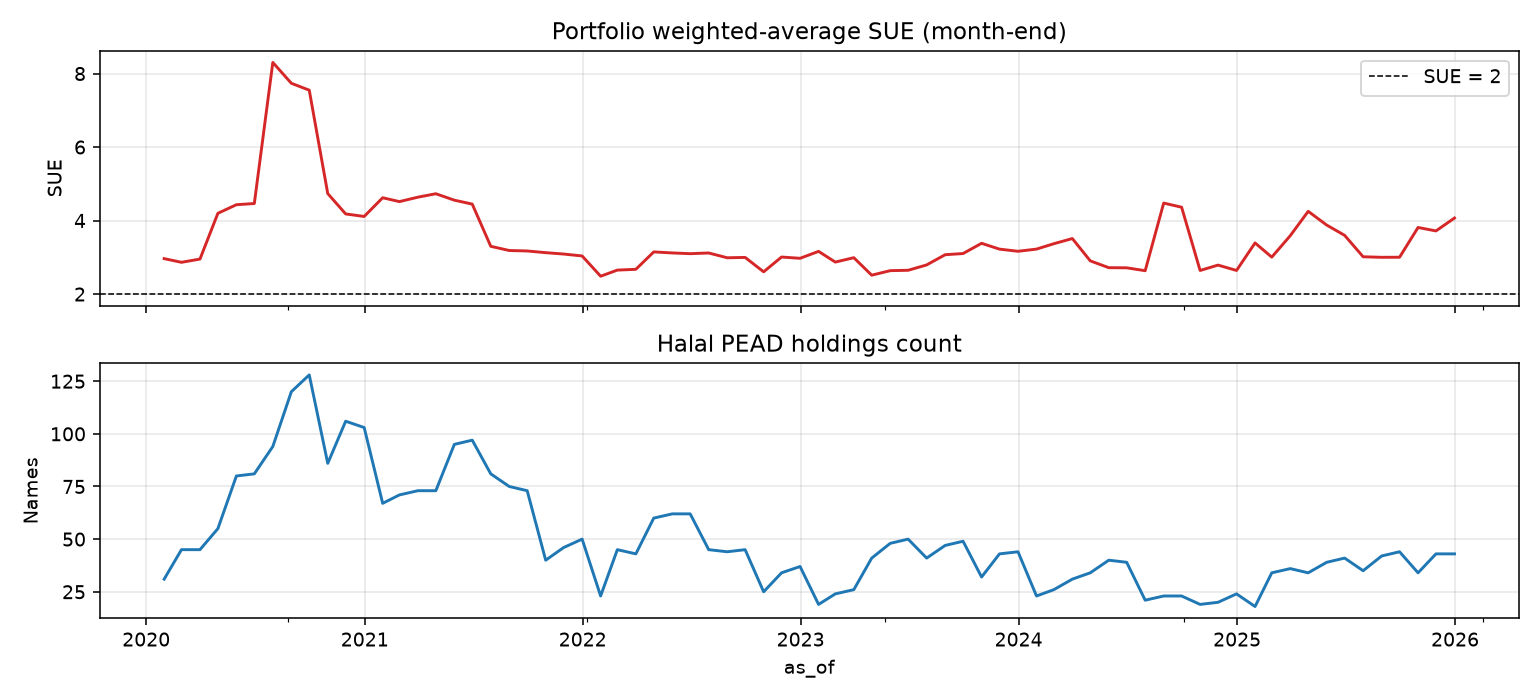
\includegraphics[width=0.88\textwidth]{figures/sue-holdings-path.png}
\caption{Average SUE of the Halal book and name count when membership changes. Holdings spike around earnings seasons and in 2020. Average SUE stays above 2 by construction, with a few extreme spikes when $\sigma$ is still tight.}
\label{fig:holdings}
\end{figure}

The book is an earnings-season sleeve, not a fully invested 50-name quality portfolio. Median 14 names, frequent trips toward a handful of positions, and a 2020 spike above 100 names are the operating reality. That is why turnover and 2025 (when fewer extreme beats may have clustered in winners) need to sit next to the CAGR.

\section{Limitations and implementation friction}
\label{sec:limits}

\subsection{Turnover, slippage, and net CAGR}

Turnover is one-way: half the $\ell_1$ weight change when event membership changes. There were 721 such changes. Average one-way turnover on those days was 20.4\% (median 15.7\%). Trading-cost drag assumes 10~basis points per one-way turn, charged on the change day.

\begin{table}[htbp]
\centering
\caption{Implementation friction on the live Halal PEAD book.}
\label{tab:friction}
\begin{tabular}{lr}
\toprule
Item & Value \\
\midrule
Membership-change events              & 721 \\
Average one-way turnover (those days) & 20.4\% \\
Assumed cost per one-way trade        & 10~bp \\
CAGR gross of trading costs           & 27.72\% \\
CAGR net of 10~bp costs               & 24.58\% \\
\bottomrule
\end{tabular}
\end{table}

Cost drag is about 3.1~points of CAGR, much larger than in the monthly quality papers in this series. Net of 10~bp the Halal book still beats SPUS (17.7\%) and SPY (15.1\%). Real slippage on names that are not mega-caps, plus crossing around earnings, could be wider. I do not model market impact, borrow, or taxes.

\begin{figure}[htbp]
\centering

\includegraphics[width=0.88\textwidth]{figures/turnover.png}
\caption{One-way turnover when PEAD membership changes. Spikes near 1.0 are full rebuilds of a small book, typical of an event sleeve.}
\label{fig:turnover}
\end{figure}

\subsection{Point-in-time compliance and survivorship}

AAOIFI tests use the latest month-end snapshot on or before the holding day, not a same-morning restatement. There is no intra-day compliance monitor. Sector exclusions use the current S\&P list and current activity labels. That is survivorship in the universe even though each print's SUE uses only prior errors.

\subsection{Data and construction issues}

Analyst consensus comes from Yahoo earnings dates, not I/B/E/S. Coverage is incomplete; 16\% of usable prints still exceed a nominal $2\sigma$ threshold, so $\sigma$ is not a textbook forecast-error scale. Split-adjusted EPS and sticky estimates remain. Several price downloads failed. GOOG/GOOGL collapse is in the live rule; other dual listings may remain. Purification of impure income is not estimated in this notebook.

The live rule was rewritten after seeing Run~1 on the same 2020--2025 window. That is in-sample specification search. A frozen rule on a later sample is the next test, not this paper.

\subsection{What this paper does not show}

There is no 2008, no hold-out after a rule freeze, no I/B/E/S-quality consensus file, and no sector-neutral twin. PEAD here is a large-cap, 21-day, equal-weight implementation. It is not Bernard and Thomas on the full CRSP file. Beating SPUS with event-time SUE in 2020--2024, then lagging in 2025, is interesting. It is not evidence that Halal PEAD is a stand-alone product.

\section{Conclusion}
\label{sec:conc}

A first, month-end, cap-weighted, 60-day SUE book lagged SPY and SPUS even though the event study showed positive drift. That was an implementation failure, not a rejection of PEAD under Halal screens. Repairing the harvest---robust SUE, one share class, equal weight, $t+1$ entry, 21-day hold---produced 27.7\% CAGR in the Halal sleeve from early 2020 through 2025, against 15.1\% for SPY and 17.7\% for SPUS. The unscreened twin returned 28.6\%. Mean 21-day CAR versus SPY is about 1.0\% for AAOIFI-compliant prints and 1.4\% for the broad index. Event-time quintiles now put Q5 above Q1.

The product shape is coherent enough to keep studying: Halal screens, a hard surprise cutoff, event-time entry, and a short hold matched to where Halal CAR actually lives. It is not ready to promote to a live mandate. Costs eat about three points of CAGR at a 10~bp assumption, the book is often thin, 2025 lagged the Halal ETF, and the $2\sigma$ screen is still not a rare tail in Yahoo data. A second paper would need a frozen rule, a proper estimate file, point-in-time index membership, explicit purification, and a sample that does not include the specification search. If Halal 21-day PEAD still beats SPUS after those steps, the claim has more to stand on. If it does not, Run~2 is mostly a demonstration that event-time implementation matters.

\paragraph{Reproduction.}
Run \texttt{code.ipynb} in this paper's folder with \texttt{FAST\_MODE=False} and dates 2020-01-01 to 2025-12-31. Live figures are in \path{figures/}. The failed first specification is archived in \path{figures/Run 1/}. The public repository is \url{https://github.com/regional-specter/Monterey-Finance}.

\bibliographystyle{plainnat}
\begin{thebibliography}{99}

\bibitem[AAOIFI(2020)]{aaoifi21}
Accounting and Auditing Organization for Islamic Financial Institutions, 2020.
\newblock Financial Paper (Shares and Bonds).
\newblock Shari'ah Standard No.~21, AAOIFI, Manama.

\bibitem[Ball and Brown(1968)]{ball1968}
Ball, R., Brown, P., 1968.
\newblock An empirical evaluation of accounting income numbers.
\newblock Journal of Accounting Research 6, 159--178.

\bibitem[Bernard and Thomas(1989)]{bernard1989}
Bernard, V.~L., Thomas, J.~K., 1989.
\newblock Post-earnings-announcement drift: Delayed price response or risk premium?
\newblock Journal of Accounting Research 27, 1--36.

\bibitem[Bernard and Thomas(1990)]{bernard1990}
Bernard, V.~L., Thomas, J.~K., 1990.
\newblock Evidence that stock prices do not fully reflect the implications of current earnings for future earnings.
\newblock Journal of Accounting and Economics 13, 305--340.

\bibitem[Derigs and Marzban(2008)]{derigs2008}
Derigs, U., Marzban, S., 2008.
\newblock Review and analysis of current Shariah-compliant equity screening practices.
\newblock International Journal of Islamic and Middle Eastern Finance and Management 1, 285--303.

\bibitem[Foster et~al.(1984)]{foster1984}
Foster, G., Olsen, C., Shevlin, T., 1984.
\newblock Earnings releases, anomalies, and the behavior of security returns.
\newblock The Accounting Review 59, 574--603.

\end{thebibliography}

\end{document}
